\documentclass[12pt,a4paper]{article}

% ===== Codificación y español =====
\usepackage[utf8]{inputenc}
\usepackage[T1]{fontenc}
\usepackage[spanish, es-tabla]{babel}

% ===== Márgenes y gráficos =====
\usepackage{geometry}
\geometry{margin=2.5cm}
\usepackage{graphicx}
\usepackage{float}        % [H] para fijar figuras/tablas
\usepackage{subcaption}   % subfiguras
\usepackage{booktabs}     % tablas más bonitas
\usepackage{amsmath}

% ===== Hipervínculos y referencias =====
\usepackage{hyperref}
\hypersetup{
  colorlinks=true,
  linkcolor=black,
  citecolor=black,
  urlcolor=blue
}

\usepackage{siunitx}
\sisetup{
  output-decimal-marker = {.}, % decimal con punto
  group-separator = {,},       % miles con coma
  group-minimum-digits = 4,
  group-digits = integer,
  table-number-alignment = center,
  round-mode = places,
  detect-all = true            % ignora configuraciones de babel
}

% Ayuda al manejo de tablas
\usepackage{tabularx}
\usepackage{adjustbox}
\usepackage{longtable}

% cleveref mejora \ref: escribe "Figura 1", "Tabla 2", etc.
\usepackage[capitalise,noabbrev]{cleveref}

% Ajuste de nombres en cleveref
\crefname{figure}{figura}{figuras}
\Crefname{figure}{Figura}{Figuras}
\crefname{subfigure}{subfigura}{subfiguras}
\Crefname{subfigure}{Subfigura}{Subfiguras}
\crefname{table}{tabla}{tablas}
\Crefname{table}{Tabla}{Tablas}
\crefname{equation}{ecuación}{ecuaciones}
\Crefname{equation}{Ecuación}{Ecuaciones}
\crefname{section}{sección}{secciones}
\Crefname{section}{Sección}{Secciones}

% Listas más controlables
\usepackage{enumitem}

\graphicspath{{figures/}}

% ===== Título y autoría =====
\title{\textbf{Clasificación no supervisada: K-Means y SOM}}
\author{Haessler Joan Ortiz Moncada \\[0.5cm]
        Universidad Distrital Francisco José de Caldas \\
        Facultad de Ingeniería \\
        Curso: Big Data}
\date{\today}

\begin{document}

\maketitle

\section{Introducción}
Este documento presenta el desarrollo de los ejercicios planteados en el \texttt{Taller\_I} 
del curso de Big Data (aunque, cronológicamente, corresponde al número 5 del curso), documentando los hallazgos 
y análisis correspondientes. Este taller se centra principalmente en el abordaje de dos \textit{\textit{datasets}}: 
uno proporcionado por el profesor de la clase, denominado \texttt{data\_clusters.mat}, y otro descargado 
de \href{https://archive.ics.uci.edu/dataset/459/avila}{Avila's dataset}. A partir de estos conjuntos de 
datos se busca implementar y practicar metodologías de clasificación no supervisada, específicamente 
K-Means y los mapas autoorganizados (SOM, por sus siglas en inglés).

\section{Metodología}
En cuanto al orden, el trabajo se desarrolla conforme a lo establecido en el \texttt{Taller\_I}. 
Respecto a la forma, la implementación de los modelos, la preparación de los datos y la visualización de 
los resultados se llevan a cabo mediante un archivo de \texttt{Jupyter Notebook} desarrollado en Colab. 
Cabe aclarar que la Inteligencia Artificial (IA) Gemini asistió en la generación del código requerido. 
Por último, el código producido, los datos implementados y el informe generado, pueden consultarse en la 
carpeta \texttt{taller\_5} del repositorio \href{https://github.com/HaesslerOrtiz/bigdata}{bigdata\_repositorio} 
de GitHub.

\section{Desarrollo}
El \texttt{Taller\_I} consta de dos ítems a desarrollar. Como es lógico, esta sección abordará en primer lugar 
el primer ítem y, posteriormente, el segundo. Para el primer ítem se requiere implementar los modelos K-Means 
y SOM sobre el dataset \texttt{data\_clusters.mat}, se permite una experimentación libre orientada únicamente 
a identificar los \textit{clusters} y la retícula de las neuronas, respectivamente.

\subsection{K\-Means con data\_clusters.mat}
Teniendo el dataset \texttt{data\_clusters.mat}, se procede a etiquetar sus dos columnas o características como 
\texttt{columnaA} y \texttt{columnaB}, así como a medir su tamaño, el cual corresponde a $135 \times 2$, donde 
ambas variables son de tipo \texttt{float}. Como regla general en este tipo de ejercicios, es recomendable estandarizar 
los datos para evitar problemas de escala entre las variables; sin embargo, debido a que los dominios de las 
características son relativamente similares, se optó por no estandarizarlas. La \Cref{fig:scatter} muestra la 
distribución de los datos del dataset.

\begin{figure}[H]
  \centering
  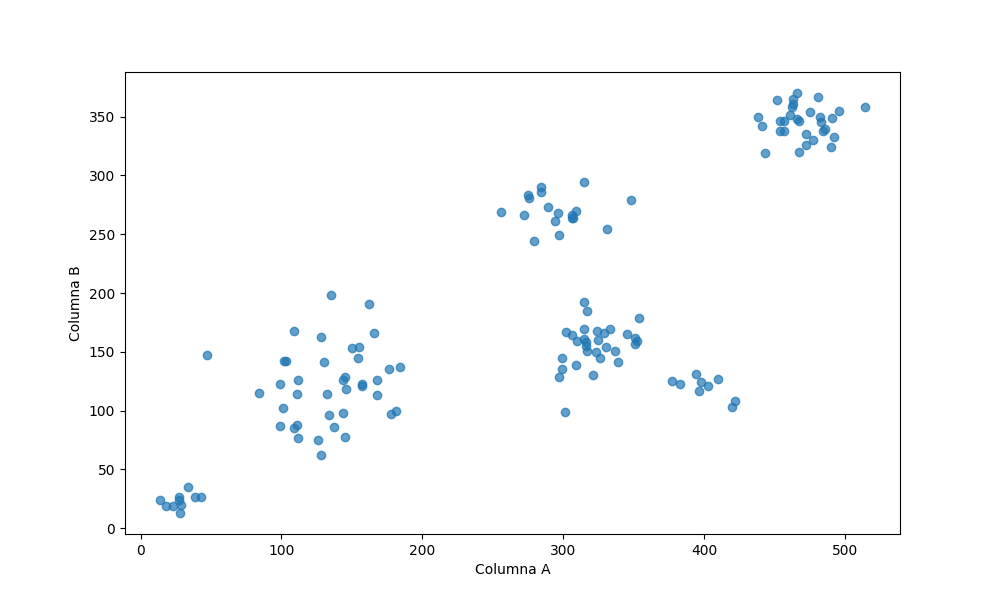
\includegraphics[width=\textwidth]{scatter_plot.png}
  \caption{Diagrama de dispersion \texttt{data\_clusters.mat}.}
  \label{fig:scatter}
\end{figure}

La \Cref{fig:scatter} permite observar que se pueden diferenciar claramente seis \textit{clusters}; sin embargo, 
para saber exactamente qué datos están asociados a ellos, se debe implementar el modelo K-means. 
El proceso propuesto es el siguiente:

\begin{enumerate}
  \item \textbf{Rango de $k$ (número de \textit{clusters}).} Entre 2 y 10.
  \item \textbf{Inicialización de los $k$ centroides.} Mediante el método \textit{k-means++}, con 50 reinicios. 
  Se mantendrá la misma semilla (\textit{Random State = 42}) para asegurar reproducibilidad. 
  Cada reinicio se entiende como una corrida independiente.
  \item \textbf{Cambio de centroides.} Mediante el método de Lloyd, con un máximo de 300 iteraciones.
  \item \textbf{Límite de iteración.} Cuando la inercia (función objetivo) no presente una variación superior a 0.0001 
  con respecto a su anterior valor en el cambio de centroides, se detendrá la iteración.
  \item \textbf{Captura de la mejor inercia.} Se registrará el valor más bajo de la inercia (función objetivo) para cada valor de $k$.
  \item \textbf{Gráfico del codo.} Con los mejores valores de inercia para cada $k$, se generará el \textit{gráfico del codo} para elegir 
  el tamaño óptimo de $k$, que corresponde al punto en el que la curva comienza a aplanarse, es decir, donde aumentar el número de clusters 
  ya no mejora sustancialmente la inercia.
\end{enumerate}

La inercia (función objetivo) se define de la siguiente forma:

\begin{equation}
  J(\{C_i\}, \{\mu_i\}) \;=\; 
  \sum_{i=1}^{k} \sum_{j=1}^{n_i} \left\| x_j^{(i)} - \mu_i \right\|^2,
  \qquad
  \mu_i = \frac{1}{n_i} \sum_{j=1}^{n_i} x_j^{(i)}.
  \label{eq:kmeans_objetivo}
\end{equation}

Donde:
\begin{itemize}
  \item $k$: número de \textit{clusters}.
  \item $C_i$: conjunto de puntos asignados al \textit{cluster} $i$.
  \item $n_i = |C_i|$: cantidad de puntos en el \textit{cluster} $i$.
  \item $x_j^{(i)}$: $j$-ésimo punto asignado al \textit{cluster} $i$.
  \item $\mu_i$: centroide del \textit{cluster} $i$, definido como el promedio de sus puntos.
  \item $\|x_j^{(i)} - \mu_i\|^2$: distancia euclídea al cuadrado entre el punto $x_j^{(i)}$ y el centroide $\mu_i$.
  \item $J$: función de inercia o función objetivo, que el algoritmo busca minimizar.
\end{itemize}

Tambien es importante mostrar como funciona el algoritmo \textit{K-means++} para elegir los centroides iniciales para cada $k$.
La inicialización de centroides se basa en la siguiente probabilidad:

\begin{equation}
  P(x) \;=\; \frac{D(x)^2}{\sum_{x' \in X} D(x')^2},
  \label{eq:kmeanspp_prob}
\end{equation}

Donde $D(x)$ es la distancia entre un punto $x$ y el centroide más cercano seleccionado hasta el momento.

El procedimiento del algoritmo \textit{K-means++} es el siguiente:

\begin{itemize}
  \item \textbf{Paso 1.} Seleccionar un primer centroide de manera aleatoria entre los puntos del conjunto de datos.
  \item \textbf{Paso 2.} Para cada punto $x$, calcular $D(x)$, la distancia entre $x$ y el centroide más cercano ya elegido.
  \item \textbf{Paso 3.} Seleccionar el siguiente centroide con probabilidad proporcional a $D(x)^2$, según la \Cref{eq:kmeanspp_prob}.
  \item \textbf{Paso 4.} Repetir los pasos 2 y 3 hasta obtener $k$ centroides iniciales.
  \item \textbf{Paso 5.} Una vez definidos los $k$ centroides iniciales, continuar con el algoritmo clásico de K-means (asignación de puntos y actualización de centroides).
\end{itemize}

La \Cref{fig:elbow} muestra el desempeño para los diferentes valores de $k$.

\begin{figure}[H]
  \centering
  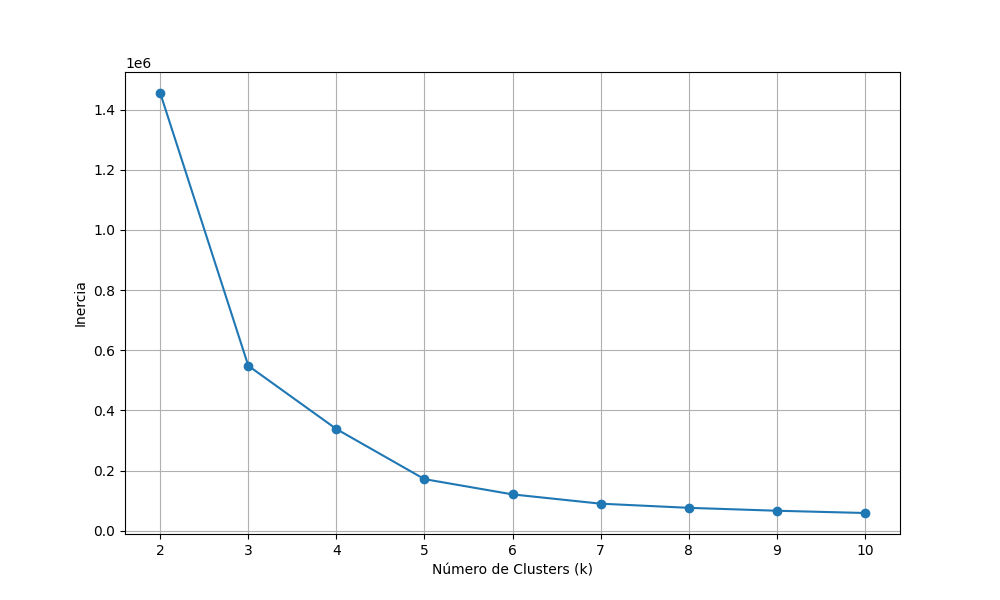
\includegraphics[width=\textwidth]{elbow_method.png}
  \caption{Diagrama del codo para \texttt{data\_clusters.mat}.}
  \label{fig:elbow}
\end{figure}

Con el gráfico anterior se concluye que el mejor valor corresponde a $k = 6$. Con esta información, se procede a 
ejecutar el modelo de \textit{K-means} con dicho valor de $k$, utilizando los mismos parámetros empleados para su 
selección. La \Cref{fig:kmeans} muestra el resultado de la ejecución de este modelo.

\begin{figure}[H]
  \centering
  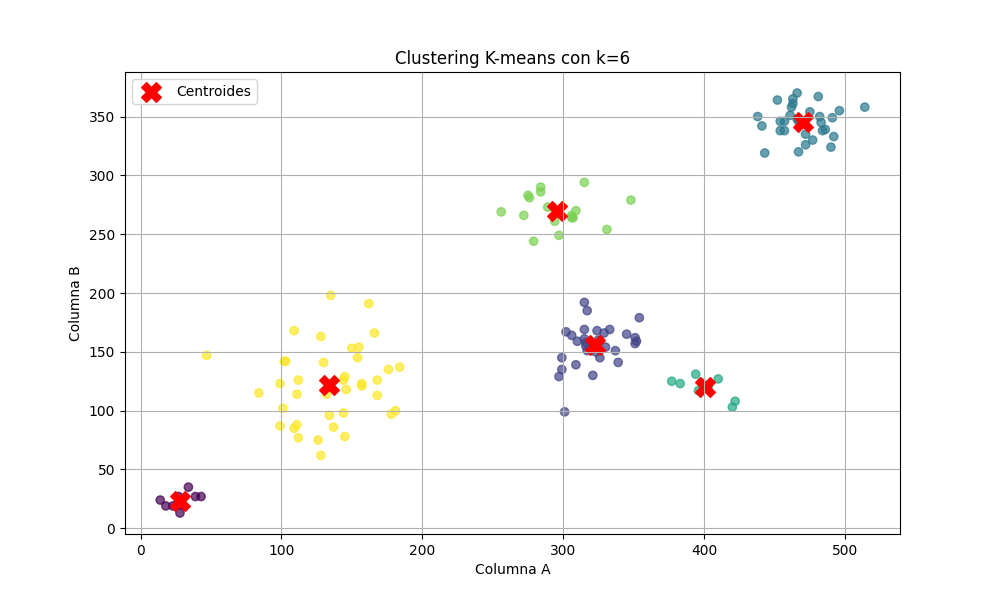
\includegraphics[width=\textwidth]{kmeans_k6_clusters.png}
  \caption{K\-means data\_clusters.mat.}
  \label{fig:kmeans}
\end{figure}

La \Cref{fig:kmeans} anterior parece haber separado correctamente los diferentes datos en sus respectivos grupos. 
No se observa ningún dato que, al menos de manera visual, se encuentre en un \textit{cluster} al que no deba pertenecer.

\subsection{SOM con data\_clusters.mat}
De una manera similar a como se procedio en la anterior seccion, se plantea la ejecucion de un algoritmo SOM 
estableciendo el siguiente flujo de ejecucion con sus respectivos hiperparámetros:

\begin{enumerate}
  \item \textbf{Estandarizar las variables.} las características se normalizan para evitar problemas de escala.
  \item \textbf{Número de épocas.} se define un total de 100 épocas, divididas en dos fases:
  \begin{itemize}
    \item \textit{Rough training:} 20 épocas con vecindad grande.
    \item \textit{Fine-tuning:} 80 épocas con vecindad pequeña.
  \end{itemize}
  \item \textbf{Retícula.} Forma cuadrada de 64 neuronas, siguiendo la regla empírica de que el número de neuronas es 
  aproximadamente $5 \cdot \sqrt{n}$, donde $n$ es el número de muestras.
  \item \textbf{Forma de vecindad.} Se adopta una topología hexagonal.
  \item \textbf{Tasa de aprendizaje.} $\alpha$ decreciente que inicia en 0.5 y puede llegar hasta un mínimo de 0.01.
  \item \textbf{Función de vecindad.} Se utiliza una función gaussiana.
  \item \textbf{Radio de vecindad.} Radio inicial igual a 4 y radio final igual a 1.
  \item \textbf{Corrección de pesos.} Los pesos se actualizan mediante la regla clásica:
  \begin{equation}
    w_i(t+1) = w_i(t) + \alpha(t) \, h_{ci}(t) \, \big( x(t) - w_i(t) \big)
  \end{equation}

  Donde:
  \begin{itemize}
    \item $h_{ci}(t)$: función de vecindad gaussiana.
    \item $w_i$: vector de pesos de la neurona $i$.
    \item $\alpha(t)$: tasa de aprendizaje en el instante $t$.
    \item $x(t)$: vector de entrada en el instante $t$.
    \item $t$: número de dato que ingresa a la retícula.
  \end{itemize}

  \item \textbf{Visualización.} Generar gráficos U-Matrix y coloreo de \textit{clusters} para observar el resultado del entrenamiento.
  \item \textbf{Evaluación.} Calcular el \textit{Quantization Error (QE)} para evaluar el rendimiento del modelo.
\end{enumerate}

El \texttt{QE} obtenido fue de 0.22, el cual, de acuerdo con la literatura, se puede considerar como un buen ajuste. 
La \Cref{fig:res_som} muestra, respectivamente, cómo se delimitan las regiones asociadas a los valores de las neuronas 
y la forma en que se van generando los \textit{clusters}, conforme a la neurona ganadora con la que se relacionan 
(los datos con el mismo color activan la misma neurona ganadora). Se observa que las neuronas ganadoras parecen clasificar 
los datos de manera muy similar a como lo hicieron los \textit{clusters} en el algoritmo \textit{k-means}.

\begin{figure}[H]
  \centering
  \begin{subfigure}[b]{0.45\textwidth}
    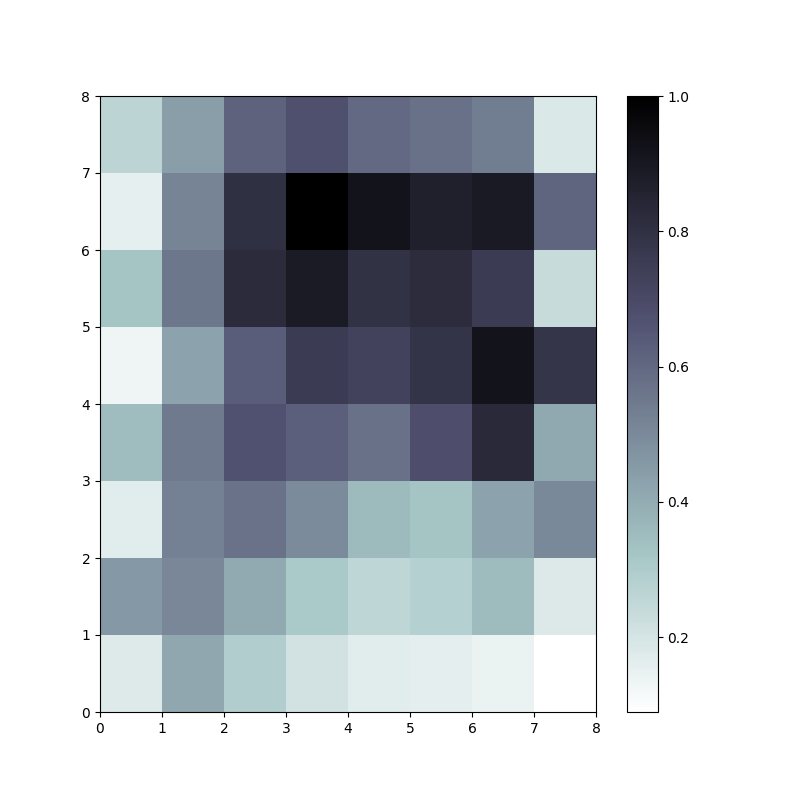
\includegraphics[width=\textwidth]{som_umatrix.png}
    \caption{Matriz de distancias/similitud.}
    \label{fig:umatrix}
  \end{subfigure}
  \hfill
  \begin{subfigure}[b]{0.45\textwidth}
    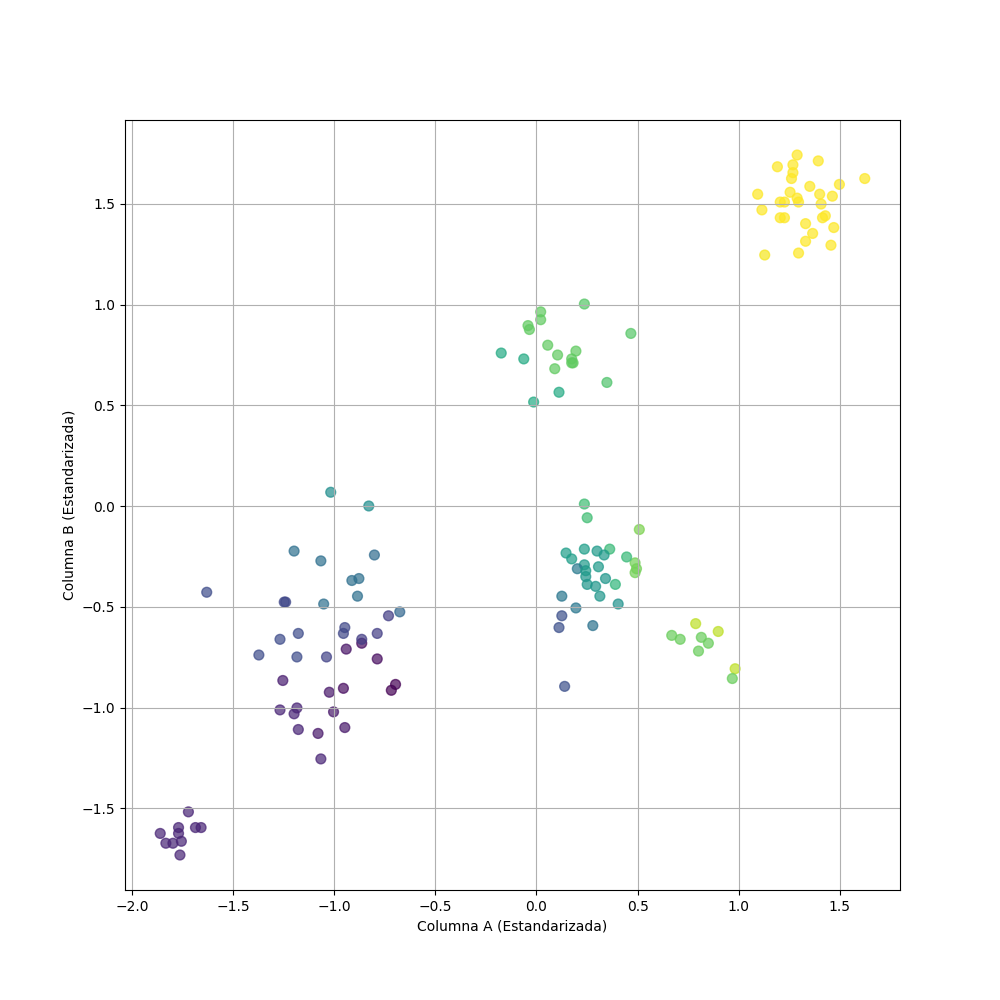
\includegraphics[width=\textwidth]{som_cluster_coloring.png}
    \caption{Activacion de neuronas}
    \label{fig:colmap}
  \end{subfigure}
  \caption{SOM resultados data\_clusters.mat.}
  \label{fig:res_som}
\end{figure}

\subsection{k-means para Avila's dataset}
El archivo que se descarga del enlace \href{https://archive.ics.uci.edu/dataset/459/avila}{Avila's dataset} contiene la siguiente 
información:

\begin{itemize}
  \item \textbf{avila-description.txt}
  \item \textbf{avila-tr.txt}
  \item \textbf{avila-ts.txt}
\end{itemize}

Los archivos \textbf{avila-tr.txt} y \textbf{avila-ts.txt} corresponden a \textit{datasets} sin encabezado 
(es decir, sin nombres en sus campos). Cada uno tiene un tamaño de 10 430 x 11, donde las columnas se dividen en 
diez características y una clase en la que se clasifican los registros. Los datos se encuentran estandarizados.

El archivo \textbf{avila-description.txt} describe el contenido de los archivos mencionados, así como el contexto 
de los datos que allí se presentan. Dichos datos registran diversas características de escritura de diferentes 
autores (cada autor corresponde a una clase).

Las características y la clase son las siguientes:

\begin{enumerate}
  \item \textbf{F2 -- Upper margin}: Margen superior.
  \item \textbf{F1 -- Intercolumnar distance}: Distancia entre columnas.
  \item \textbf{F3 -- Lower margin}: Margen inferior.
  \item \textbf{F4 -- Exploitation}: Grado de explotación o uso del espacio.
  \item \textbf{F5 -- Row number}: Número de filas.
  \item \textbf{F6 -- Modular ratio}: Relación modular.
  \item \textbf{F7 -- Interlinear spacing}: Espaciado entre líneas.
  \item \textbf{F8 -- Weight}: Peso.
  \item \textbf{F9 -- Peak number}: Número de picos.
  \item \textbf{F10 -- Modular ratio / Interlinear spacing}: Relación entre el módulo y el espaciado interlineal.
  \item \textbf{Clase}: Variable categórica que puede tomar los valores \texttt{A, B, C, D, E, F, G, H, I, W, X, Y}.
\end{enumerate}

Antes de implementar el algoritmo \texttt{k-means}, se eliminaron los registros correspondientes a las cuatro clases menos 
frecuentes, tal como se indica en el \texttt{Taller\_I}. En concreto, se excluyeron los registros pertenecientes a las 
clases \texttt{B, C, W} y \texttt{Y}. Adicionalmente, se asignaron nombres a las columnas de acuerdo con lo definido en el 
archivo \textbf{avila-description.txt}. Tras la eliminación de registros, los tamaños de los \textit{datasets} 
\textbf{avila-tr.txt} y \textbf{avila-ts.txt} quedaron en $10012 \times 11$ y $10017 \times 11$, respectivamente.

Para ejecutar el algoritmo \texttt{k-means} se utilizó un enfoque similar al aplicado anteriormente, con la diferencia de 
que se modificaron el número de corridas y el rango de valores de $k$ a probar. En este caso, se establecieron 50 corridas 
y un rango de $k$ entre 2 y 25. Con la configuración recién descrita, se obtuvo el siguiente gráfico del codo.

\begin{figure}[H]
  \centering
  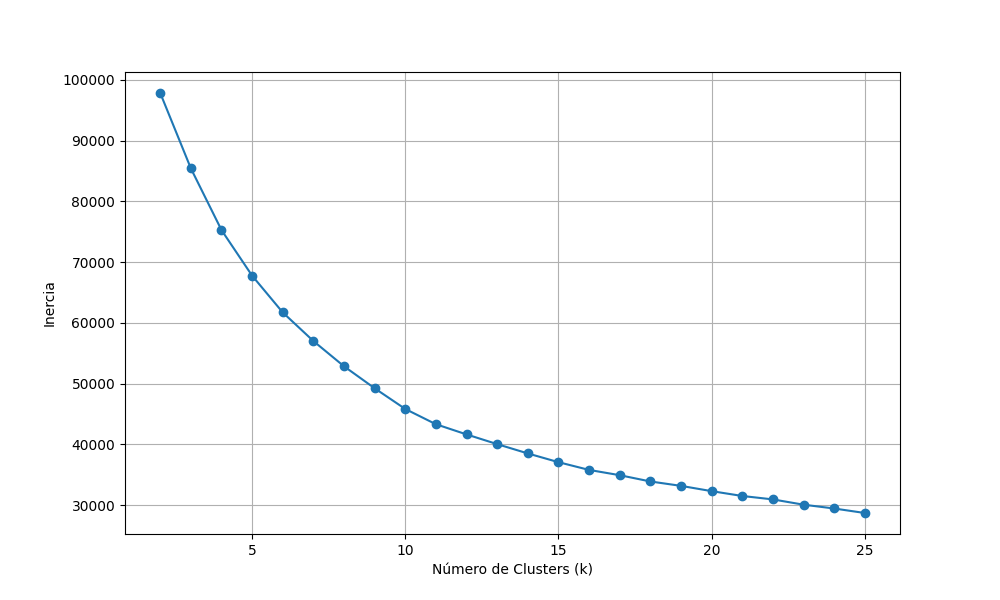
\includegraphics[width=\textwidth]{elbow_method_tr_filtered.png}
  \caption{Diagrama del codo para \texttt{Avila's dataset}.}
  \label{fig:elbow2}
\end{figure}

Con el mismo criterio utilizado para seleccionar el valor óptimo de $k$ en el \texttt{k-means} anterior, se determinó que 
$k = 15$ era la mejor elección para este caso. Una vez en este punto ya se puede ejecutar el modelo con la misma 
configuración con la que se eligio el valor de k.

Con el modelo \texttt{k-means} ejecutado, se procede a realizar un proceso de vinculación mediante el cual a cada uno de los 
\textit{clusters} generados se le asigna una clase. Esta asignación se realiza con base en la clase mayoritaria dentro de 
cada \textit{cluster}; es decir, se asigna a un \textit{cluster} la clase que más lo representa según la mayor cantidad de 
registros clasificados en él. Cabe aclarar que en ningún momento se utilizó la información de las clases existentes en los 
\textit{datasets} para la generación de los \textit{clusters}; la relación entre clases y resultados de \texttt{k-means} se 
estableció mediante el mapeo posicional de cada dato con su respectiva clase en el \textit{dataset} original. Para este 
proceso se empleó el \textit{dataset} generado a partir de la información contenida en el archivo \textbf{avila-tr.txt}.

Con base en lo anterior, es posible generar una matriz de confusion que permita analizar con que precision el algoritmo 
k-means esta clasificando a las diferentes clases del dataset \textbf{avila-tr.txt}. Esto se puede ver en la 
Figura a continuacion: 

\begin{figure}[H]
  \centering
  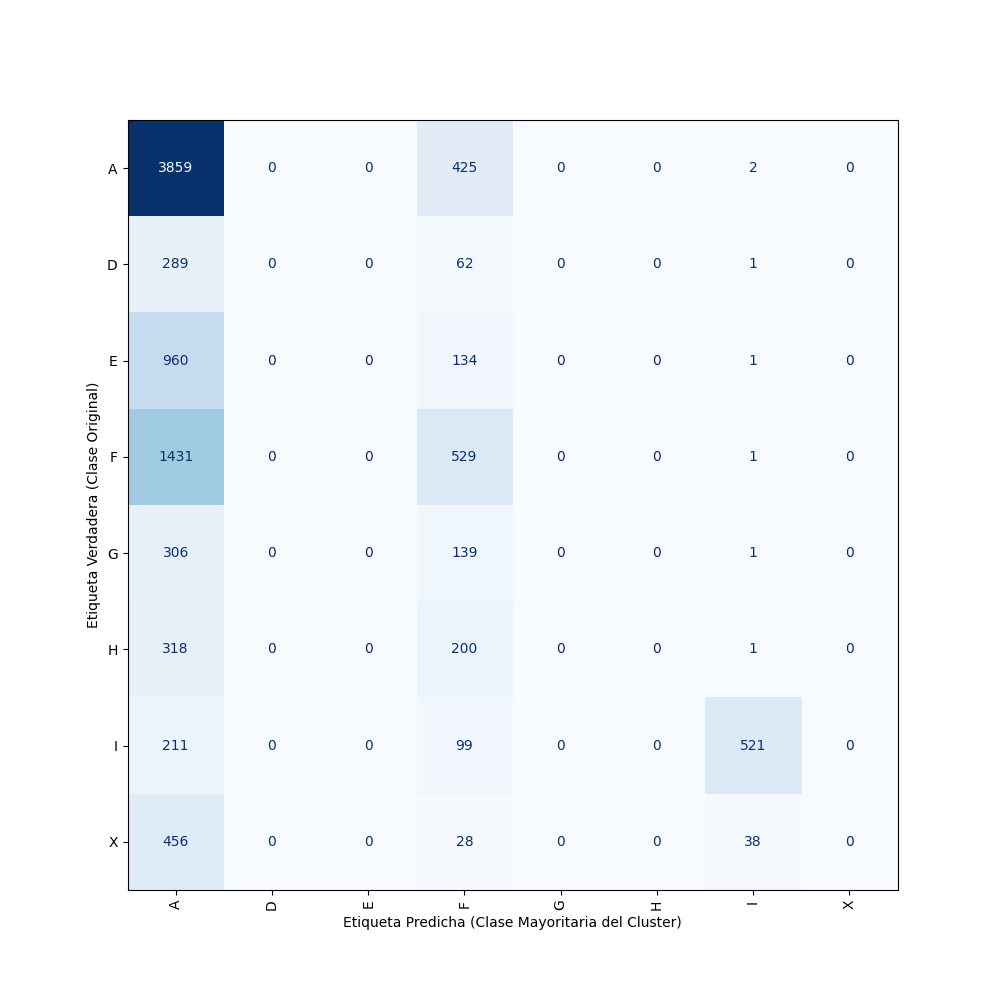
\includegraphics[width=\textwidth]{confusion_matrix_kmeans_k15.png}
  \caption{Matriz de confusion para k-means semisupervisado para el\texttt{Avila's dataset}.}
  \label{fig:mat_confux_kmeans}
\end{figure}

Observando la Figura anterior se concluye que el algortimo \texttt{k-means} solo clasifica tres clases:
\texttt{A, F, I}, teniendo baja exactitud, pues arroja muchos falsos positivos (especialmente en la clase \texttt{F}), y 
tiende a confundir mucho la clase \texttt{A} con la clase \texttt{F}, aunque parece gozar de cierta exactitud al clasificar 
la clase \texttt{I}. Como conclusion se puede afirmar que el algoritmo \texttt{k-means} ejecutado tiene un desempeño muy bajo.

Realizando una validacion cruzada del algoritmo en cuestion con el dataset del archivo \textbf{avila-ts.txt}, se tiene el 
siguiente resultado:

\begin{figure}[H]
  \centering
  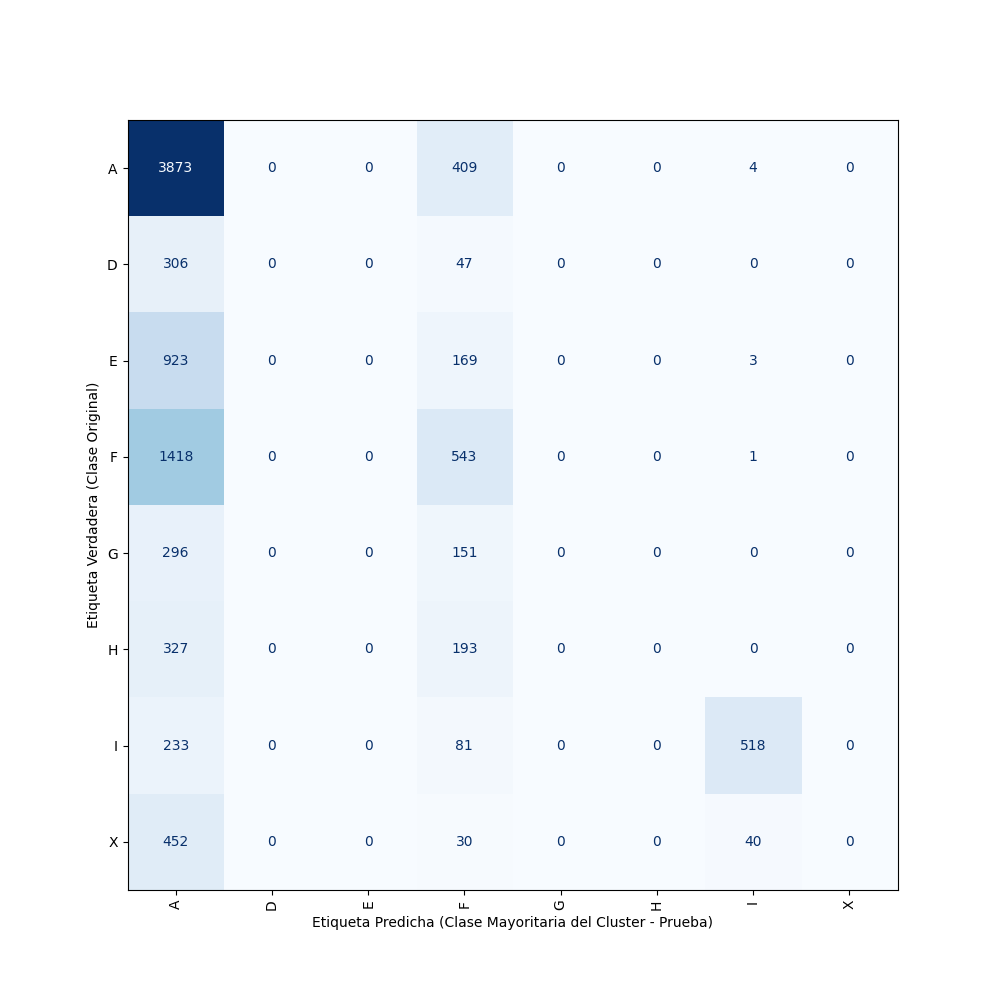
\includegraphics[width=\textwidth]{confusion_matrix_kmeans_k15_test.png}
  \caption{Matriz de confusion para k-means semisupervisado para el \texttt{Avila's dataset} dataset de test.}
  \label{fig:mat_confux_kmeans_test}
\end{figure}

Como lo muestra la \Cref{fig:mat_confux_kmeans}, el algoritmo \texttt{k-means} presenta un desempeño muy similar 
tanto en el \textit{dataset} de entrenamiento como en el de prueba.

\subsection{SOM para Avila's dataset}
Para ejecutar el algoritmo \texttt{SOM} se utilizó un enfoque similar al aplicado anteriormente, con la diferencia de que 
se probaron distintos tamaños de retículas. El rango elegido fue entre $16 \times 16$ y $36 \times 36$ neuronas. 
Se definió una tasa de aprendizaje que inicia en 0.4 y finaliza en 0.2, un radio de vecindad variable de acuerdo con el 
tamaño de la retícula evaluada, y se empleó un algoritmo de aprendizaje \texttt{batch SOM}, el cual funciona de manera 
similar al mecanismo tradicional de corrección de pesos del SOM, pero en lugar de ajustar los pesos de las neuronas en cada 
entrada, realiza la corrección en bloque; es decir, con todos los datos que ingresan en una época. Los resultados del 
entrenamiento (ver \Cref{fig:QE}) permiten concluir que la retícula de tamaño $29 \times 29$ es la que arroja el mejor 
desempeño en relación con el valor de \texttt{QE}.

\begin{figure}[H]
  \centering
  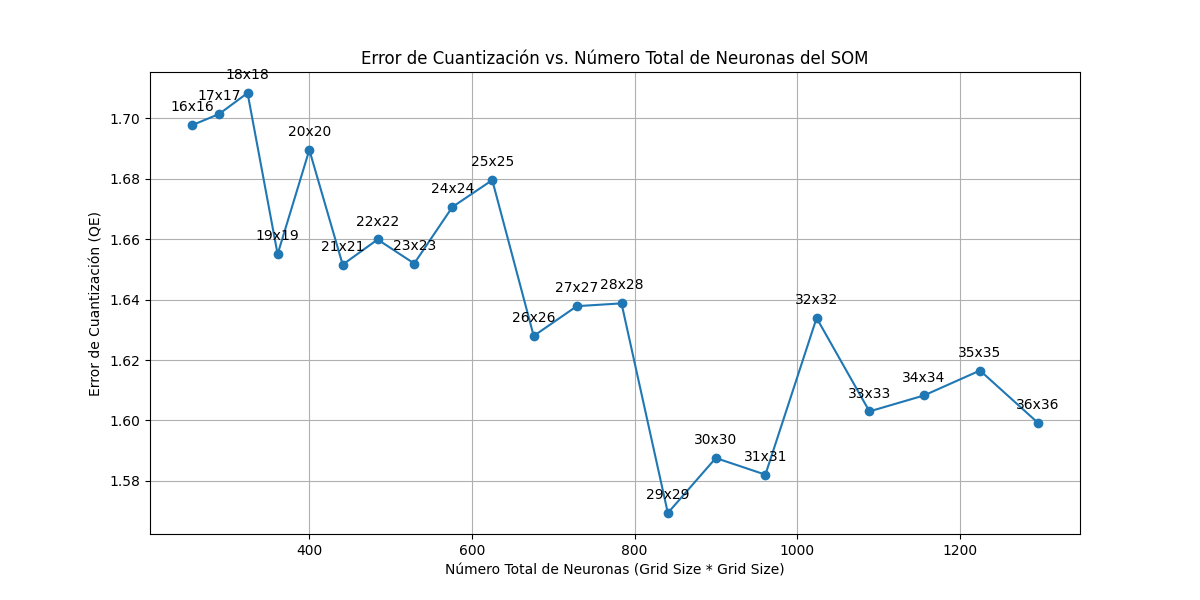
\includegraphics[width=\textwidth]{som_qe_vs_neurons.png}
  \caption{\texttt{QE} versus tamaño de reticula.}
  \label{fig:QE}
\end{figure}

Teniendo el tamaño óptimo de la retícula, de acuerdo con el entrenamiento realizado sobre el \textit{dataset} de 
entrenamiento, se procede a ejecutar el modelo \texttt{SOM}. De manera similar a lo realizado con el algoritmo 
\texttt{k-means}, se genera un mapeo de los datos con su respectiva clase, y se construye una matriz de confusión 
(ver \Cref{fig:QE}) que permite evaluar el desempeño del modelo y adicionalmente se tienen las siguientes métricas: 

\begin{table}[H]
    \centering
    \begin{tabular}{|l|c|}
        \hline
        \textbf{Métrica} & \textbf{Valor} \\ \hline
        Accuracy                 & 0.5574 \\
        F1-Score (Ponderado)     & 0.5007 \\
        Precisión (Ponderado)    & 0.5426 \\
        Recall (Ponderado)       & 0.5574 \\ \hline
    \end{tabular}
    \caption{Métricas de clasificación SOM dataset de entrenamiento.}
    \label{tab:metricas_clasificacion}
\end{table}

\begin{figure}[H]
  \centering
  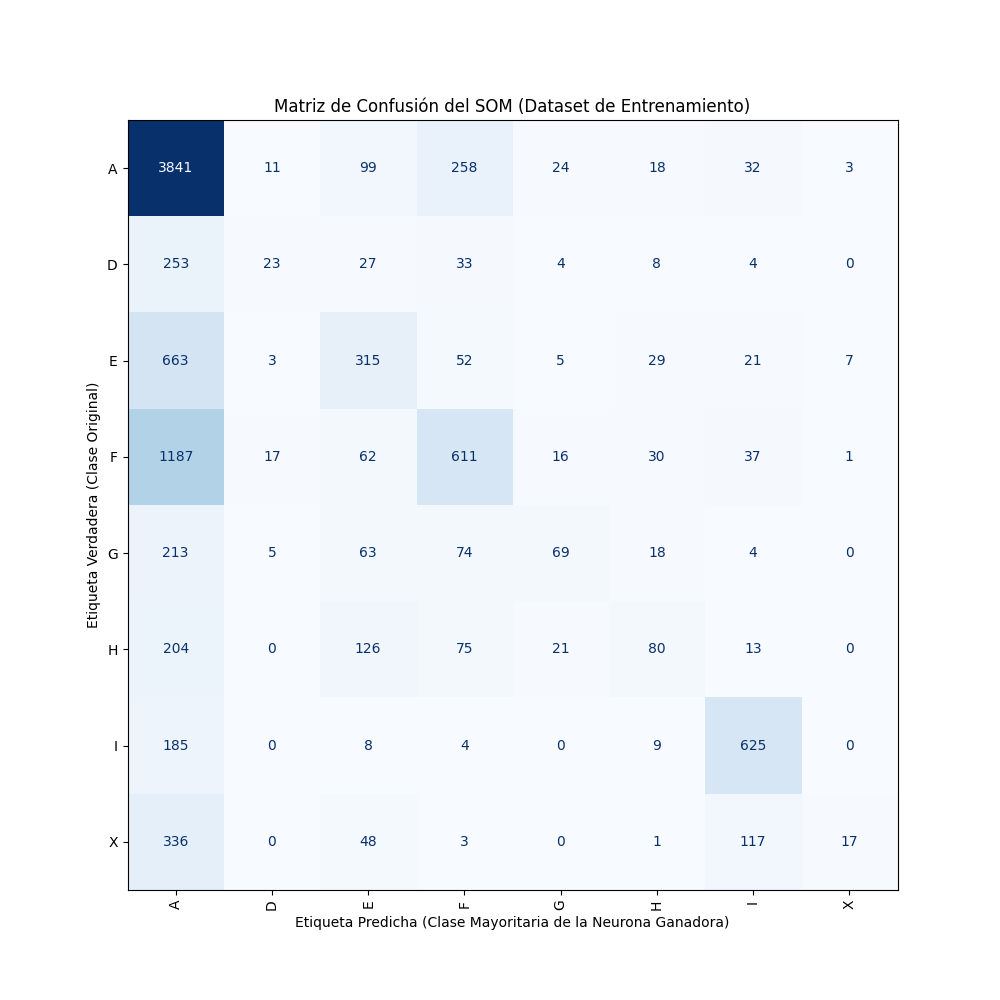
\includegraphics[width=\textwidth]{confusion_matrix_som_train.png}
  \caption{Matriz de confusion para SOM semisupervisado para el dataset de entrenamiento.}
  \label{fig:mat_confux_SOM_train}
\end{figure}

Analizando los resultados, se observa que el modelo presenta un desempeño limitado. Sin embargo, en contraste con el 
algoritmo \texttt{k-means}, el modelo \texttt{SOM} logra capturar un mayor número de clases, aunque aún con bajo rendimiento; 
incluso consigue identificar todas las clases del \textit{dataset}. Es posible que, con un \textit{dataset} más balanceado, 
el modelo \texttt{SOM} pueda ofrecer mejores resultados. Asimismo, sería interesante probar un análisis de características 
previo a su uso en el modelo, ya que algunas variables podrían no estar aportando información relevante, generar ruido 
o presentar colinealidad con otras.

También se hizo un proceso de validación cruzada en donde se probó el modelo entrenado \texttt{SOM}, con los datos del 
dataset del archivo \textbf{avila-ts.txt}. Se obTUVO el siguiente resultado:

\begin{figure}[H]
  \centering
  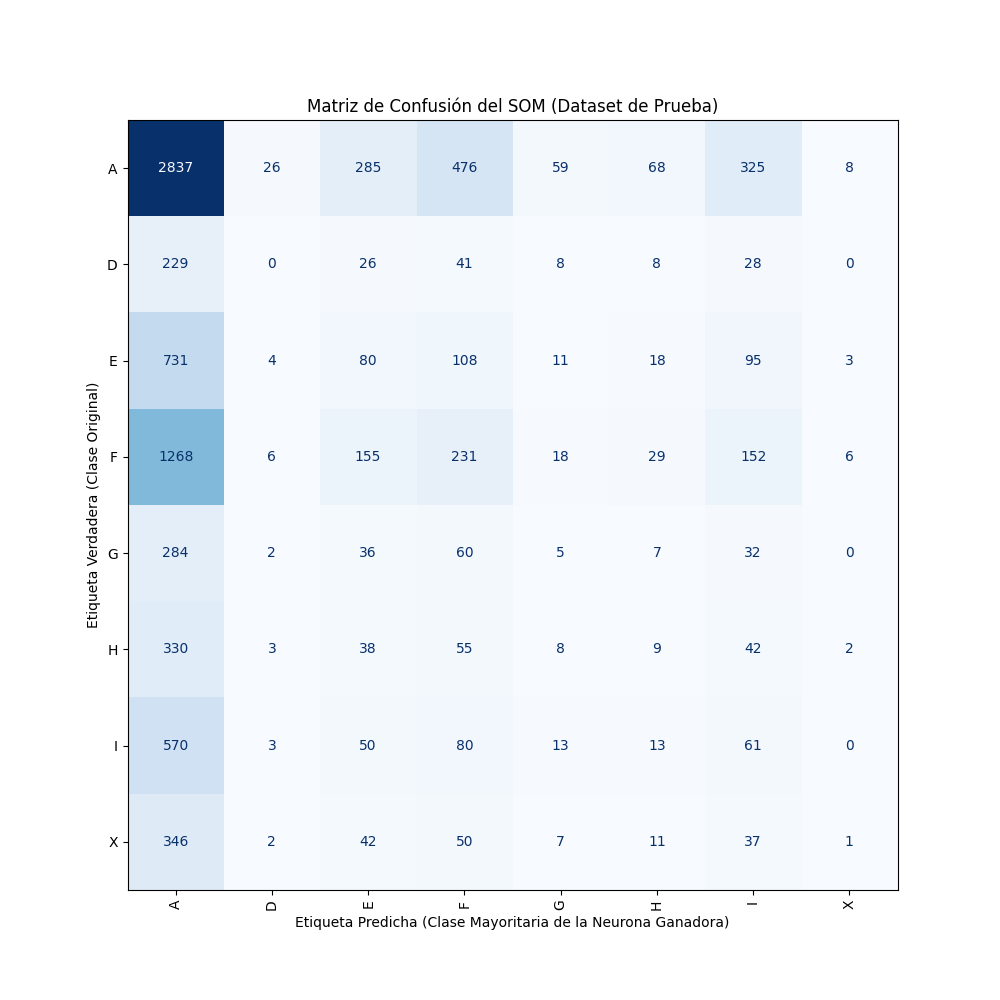
\includegraphics[width=\textwidth]{confusion_matrix_som_test.png}
  \caption{Matriz de confusion para SOM semisupervisado para el dataset de test.}
  \label{fig:mat_confux_SOM_test}
\end{figure}

La \Cref{fig:mat_confux_SOM_test} arroja que el modelo se comporta de manera muy similar a como se comportó en 
el conjunto de entrenamiento.
\end{document}